\begin{frame}
\section{}
Consider this model:

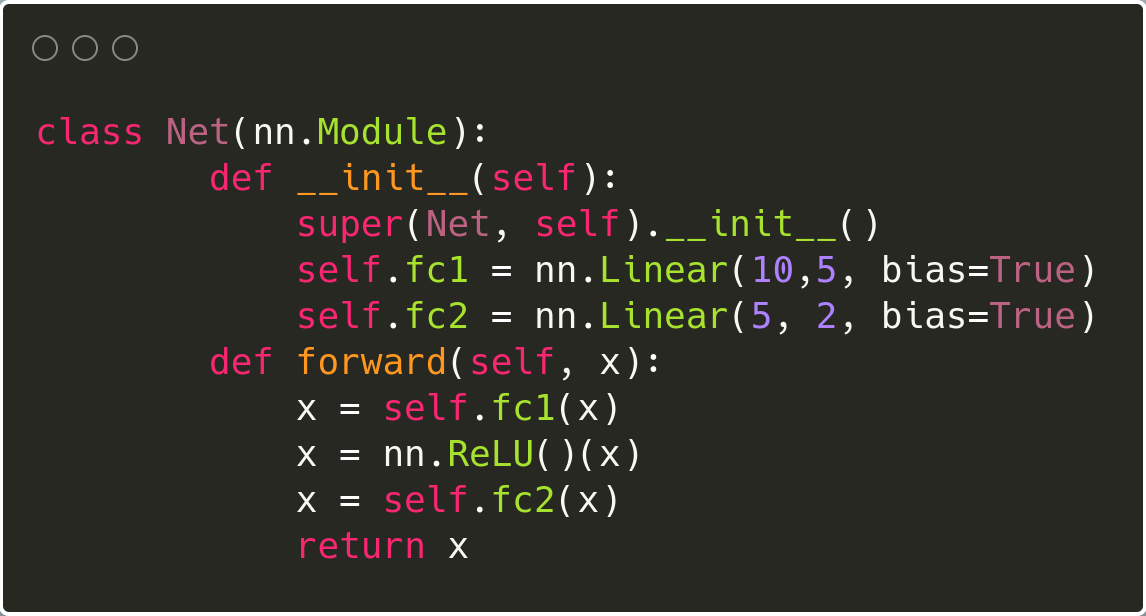
\includegraphics[scale=0.2]{images/q33_1.png}

What is the number of trainable parameters in this model
\begin{enumerate}[label=(\Alph*)]
\item Depends on the input
\item 60
\item 62
\item 67    % Ans
\item None of these   % None
\end{enumerate}
\end{frame}

\begin{frame}
\section{}
Consider this model:

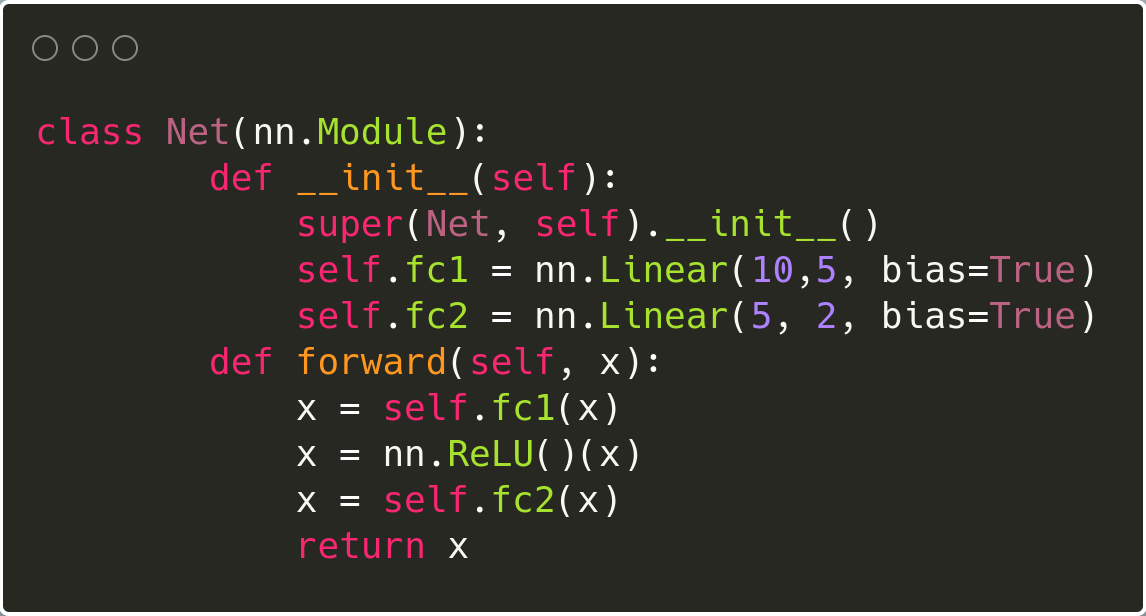
\includegraphics[scale=0.2]{images/q33_2.png}

Now consider that a tensor of shape $(5,10)$ is given as input to this model. What is the shape of the output tensor?
\begin{enumerate}[label=(\Alph*)]
\item $(10,2)$
\item $(5,2)$    % Ans
\item $(5,5)$
\item Cannot be answered with given information
\item None of these   % None
\end{enumerate}
\end{frame}

\begin{frame}
\section{}
Consider this model:

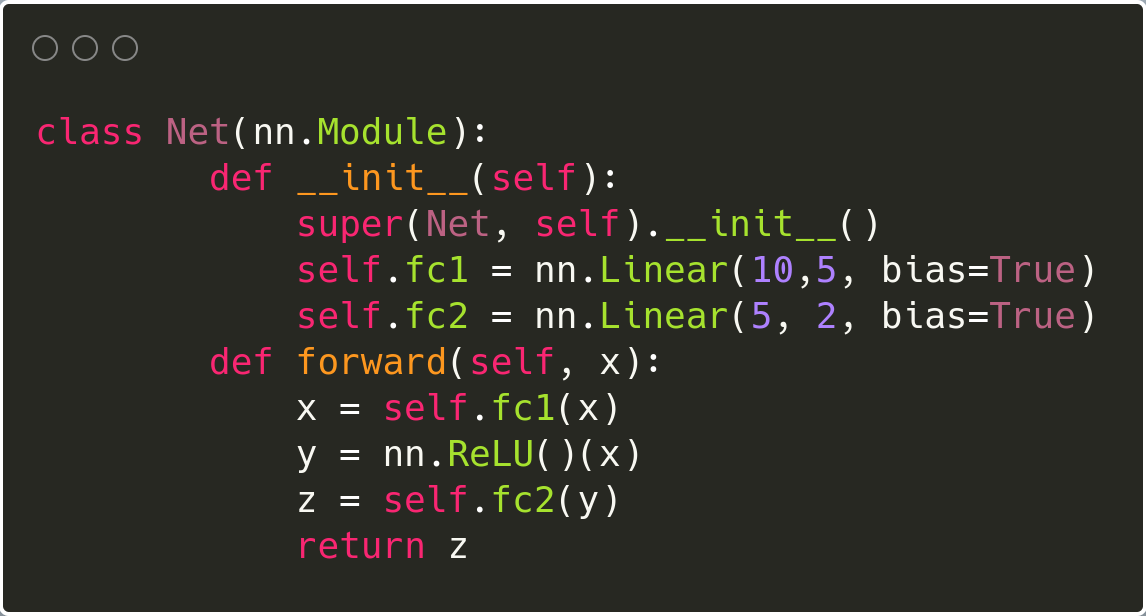
\includegraphics[scale=0.2]{images/q33_3.png}

Now consider that a tensor of shape $(5,10)$ is given as input to this model. What is the shape of the tensor y in the forward function ?
\begin{enumerate}[label=(\Alph*)]
\item $(10,2)$
\item $(5,2)$
\item $(5,5)$   % Ans
\item Cannot be answered with given information
\item None of these   % None
\end{enumerate}
\end{frame}


\begin{frame}
\section{}
Which of these are valid ways to address the problem of overfitting?
\begin{enumerate}[label=(\Alph*)]
\item Data augmentation   % Ans
\item L1 regularization of weights    % Ans
\item Increase the number of layers in model
\item Decrease the number of layers in model    % Ans
\item Add dropout to one of the layers    % Ans
\item None of these  % None
\end{enumerate}
\end{frame}


\begin{frame}
\section{}
Consider this model with just 1 convolutional layer.

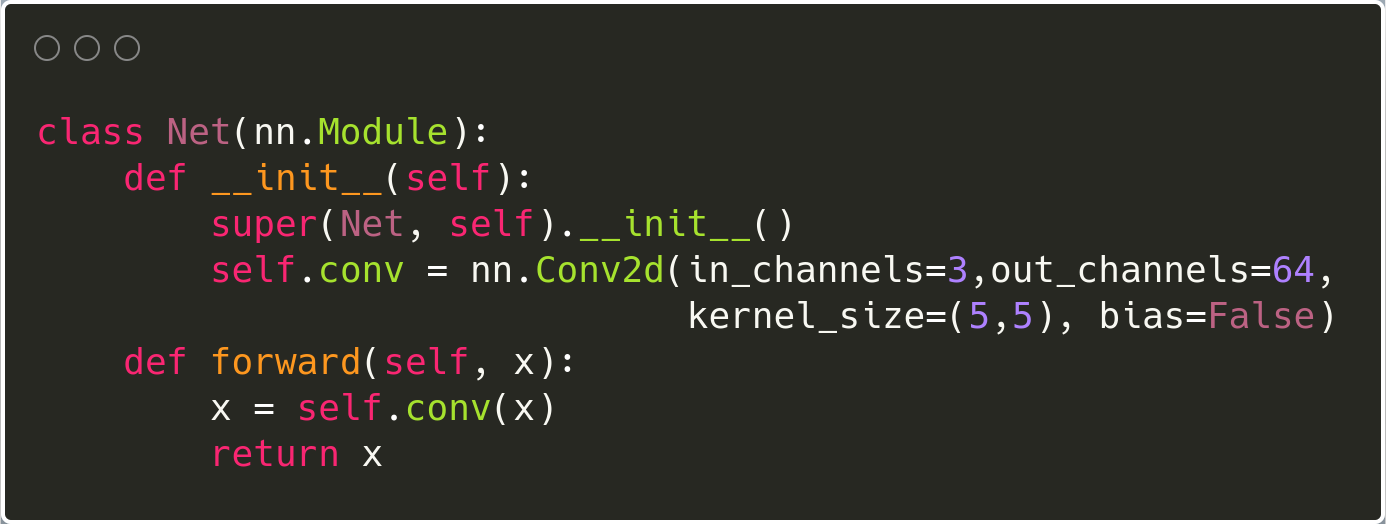
\includegraphics[scale=0.2]{images/q33_5.png}

Consider that we want to input a tensor of shape (10,3,512,512) to this model. Then

\begin{enumerate}[label=(\Alph*)]
\item The number of trainable parameters is $64\times5\times5$
\item The number of trainable parameters is $64\times3\times5\times5$   % Ans
\item The shape of output tensor is $(10,3,508,508)$
\item The shape of output tensor is $(10,64,508,508)$   % Ans
\item None of these   % None
\end{enumerate}
\end{frame}
